\chapter{Architecture of Wireless Communication Active Balancing BMS}\label{ch:Architecture_Active_Balancing_BMS}
\section{Introduction}
There are plenty of topologies dedicated to the BMS active balancing, for instance, cell-to-cell charge balancing, cell-to-stack or stack-to-cell charge sharing, and stack charge sharing. Among such wide techniques cell to stack and stack-cell, charge-sharing techniques gain the upper hand because of their robustness and safety measures against the battery.
\section{Active Balancing Topologies for BMS }

\subsection{\textit{Type Ia} : Combination of Buck and Boost Converter}

\subsection{\textit{Type Ia} : Combination of the Buck/Boost Converter :}
The figure\ref{fig:Type 1a Active Battery Balancing} illustrates the Type Ia balancing method for a battery system with n series-connected cells. The description is stack-to-cells-to-stack in accordance with the accepted nomenclature. A buck converter serves as a charging unit that distributes charge from the stack to the chosen cells. A boost converter reverses the process of discharge.
\\
The boost converter's input and output voltage ranges must be large enough to accommodate cells with voltages ranging from 1 to n-1. All cells can be actively charged and discharged up to the top level of the stack in this manner. It is only possible for nearby cells to balance numerous cells at once. Access to all cells below the topmost cell is used to balance that cell.
\\
This section explains the balancing procedure shown in Figure \ref{fig:Type 1a Active Battery Balancing}. The buck converter feeds Cell 1 with energy from the stack through switch \textit{$S_wA1$}. The converter output current $I_{Buck}$ is used to charge Cell 1. With the converter input current boost, the boost converter simultaneously discharges Cell 1 and Cell 2 through \textit{$S_wB2$}. The sum of the current in Cell 1 is 0A since $I_{Buck} = -I_{Boost} = I_{Bal}$, while Cell 2 discharges with $I_{boost}$A (negative balancing or "discharge mode"). The buck converter is often connected higher than the boost converter Batteries in Charging Mode. Discharging is done in the opposite order.
\\

\begin{figure}[h]
	\centering
	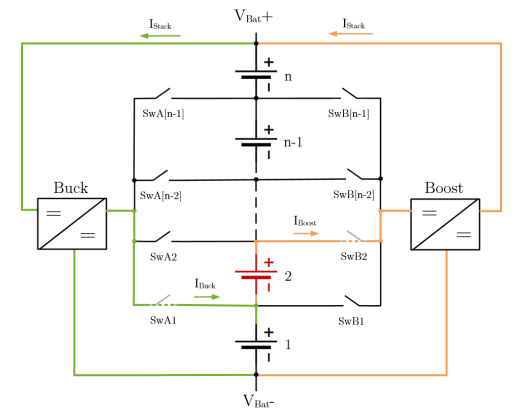
\includegraphics[width=0.7\textwidth]{Chap04/Figures/Type1a_ABMS.PNG}
	\caption{\textit{Type Ia}: Active Battery Balancing} 
	\label{fig:Type 1a Active Battery Balancing}
\end{figure}

The idle cell currents can be expressed as a vector following \ref{eq:Type1_cell_current}. It accounts for the balancing currents, both positive and negative, as well as the resulting stack current.
\begin{equation}\label{eq:Type1_cell_current}
    \vec{I_{Cell}}  = I_{stack} + \vec{I_n}\centerdot I_{Bal} - \vec{OUT}\centerdot I_{Bal}
\end{equation}

\begin{equation}\label{eq:Type1_cell_current}
    I_{stack}  = I_{Bal}(\frac{1}{\eta } \sum_{}^{}\vec{I_n}  - \eta\sum \vec{Out} ) \\
\end{equation}

\begin{equation}
\vec{OUT}  = \begin{pmatrix}
    S_{B1}\\
    \vdots
    S_{B[n-1]}  
\end{pmatrix} \\
, S_{x}=\left\{0\cdots1\right\}\\
, \vec{I_n}  = \begin{pmatrix}
    S_{A1}\\
    \vdots
    S_{A[n-1]}
\end{pmatrix} \\
\end{equation}

where $\vec{I_n}$ and $\vec{OUT}$ are the vectors of the switch signals $S_{A[x]}$ and $S_{B[x]}$ , respectively.
\\
The converter power and overall losses depend on the stack's n cells and the location of the balanced cell inside it. They rise as the position and the number of cells increases. \textit{I = J} when a single cell is in balance, In the absence of that, \textit{I} stands for the bottom cell of the balancing group and \textit{j} for the top one. As a result, \textit{I} and \textit{j} is always true.
\\
The necessary converters can be the traditional buck and boost converters depicted in Figures \ref{fig:Conventional Buck (a) and synchronous Buck(b) Conveter} and \ref{fig:Conventional Boost (a) and synchronous Boost(b) Conveter}. A synchronous design can be adopted, in which the diode is replaced with an actively regulated MOSFET to eliminate losses and to improve the efficiency of the converters across the whole operating range.
\begin{figure}[h]
	\centering
	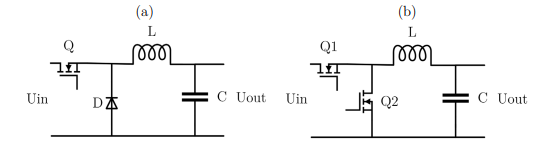
\includegraphics[width=0.9\textwidth]{Chap04/Figures/Conventiaonal_buck_synch_buck.PNG}
	\caption{Conventional Buck (a) and synchronous Buck(b) Conveter} 
	\label{fig:Conventional Buck (a) and synchronous Buck(b) Conveter}
\end{figure}

\begin{figure}[h]
	\centering
	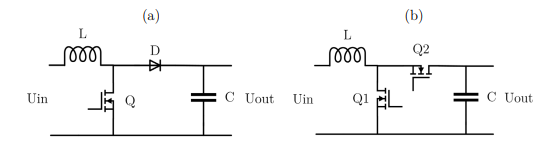
\includegraphics[width=0.9\textwidth]{Chap04/Figures/Conventiaonal_boost_synch_boost.PNG}
	\caption{Conventional Boost (a) and synchronous Boost(b) Conveter} 
	\label{fig:Conventional Boost (a) and synchronous Boost(b) Conveter}
\end{figure}

\subsection{\textit{Type Ib} : \textit{Type Ia} with a bidirectional converter :}
In terms of balancing routes, \textit{Type Ib} is comparable to \textit{Type Ia}. Bidirectional converters are used in place of unidirectional ones. Figure \ref{fig:Type1b Active Balancing Circuit } depicts the schematic for potential hardware implementation.\\

\subsection{\textit{Type IIa} :  Buck-boost converter :}
The Type IIa of the discussed balancing techniques is shown in Figure 50. Once more, n cells are arranged in series to make up the battery system. The description is cells-to-cells following the accepted nomenclature. This approach is comparable to cell bypassing if the load current and balancing current are the same. In discharge mode, a buck converter moves charge from one cell or many neighboring cells to its subjacent cells in the stack. A boost converter transfers charge in the other direction when it is in charge mode. A single bidirectional buck-boost converter can be created by combining the two converters.
\begin{figure}[h]
	\centering
	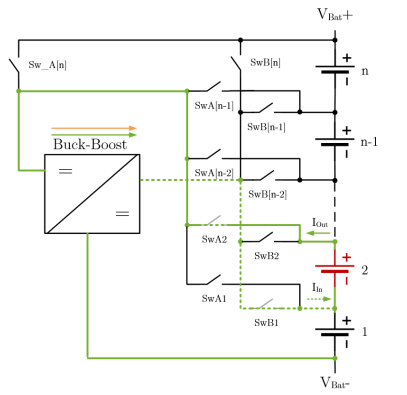
\includegraphics[width=0.6\textwidth]{Chap04/Figures/Type2a_ABMS.PNG}
	\caption{\textit{Type IIa} :  Buck-boost converter }
	\label{fig:Type2a Buck-boost converter}
\end{figure}
A bidirectional buck-boost converter made up of both converters is possible. To support 1 to n cells, the buck-boost converter's input and output voltage ranges must be sufficiently broad. Only cells that are close to one another can balance numerous cells at once. 
\\
\indent The explanation for the balancing procedure shown in Figure \ref{fig:Type2a Buck-boost converter} is given in the paragraphs that follow. Switches $S_{wA[2]}$ and $S_{wB[1]}$ in the buck converter allow the energy from Cells 1 and 2 to be transferred to Cell 1. 
it releases cells 1 and 2. The converter output current $I_{In}$ charges cell number one. In turn, Cell 1 is charged with $(I_{In} - I_{Out})$ A while Cell 2 is discharged with $I_{Out}$ A (negative balancing). $I_{Out}$ becomes $I_{Bal}$. 
In most cases, charging occurs when the DC/DC converter is connected in parallel to the desired cells and is in boost mode. However, in buck mode, discharge is performed in the same manner. Same charge and discharge operations as with \textit{Type I} are possible through switches $S_{wA[n]}$ and $S_{wB[n]}$.
\\
Depending on the number of balanced cells, the resulting cell current can be expressed as a vector:
\begin{equation}\label{eq:Type2_cell_current}
    \vec{I_{Cell}}  = \vec{I_{n}} \centerdot I_{Bal}  + \eta \centerdot \frac{\sum \vec{I_{n}}}{\sum \vec{I_{Out}}}\centerdot \vec{I_{Out}} \centerdot I_{Bal}
\end{equation}
\begin{equation}
    \vec{OUT}  = \begin{pmatrix}
        S_{B1}\\
        \vdots
        S_{Bn}  
    \end{pmatrix} \\
    , S_{x}=\left\{0\cdots1\right\}\\
    , \vec{I_n}  = \begin{pmatrix}
        S_{A1}\\
        \vdots
        S_{An}
    \end{pmatrix} \\
\end{equation}

\begin{figure}[h]
	\centering
	\subfigure[Conventional Buck-Boost Converter]{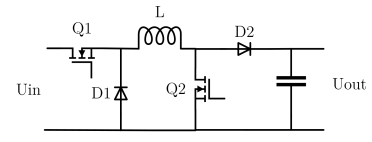
\includegraphics[scale=.7]{Chap04/Figures/Buck_boost_conventional.PNG}}
	\qquad
	\subfigure[Synchronous Buck-Boost Converter]{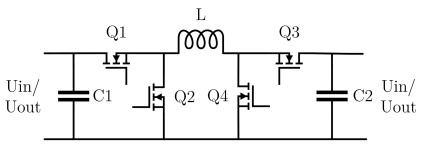
\includegraphics[scale=.7]{Chap04/Figures/Synchronous_buck_boost.PNG}}
	\caption{Typical Buck-Boost Converters}
	\label{fig:Type2a Typical Buck boost}
\end{figure}
Figure \ref{fig:Type2a Typical Buck boost}(a) depicts a potential buck-boost converter implementation. The N-MOSFET Q2 is disabled for buck mode, and Q1 is turned on and off. Q1 is constantly on in boost mode while Q2 is actively switched. The four-switch buck-boost converter from Figure \ref{fig:Type2a Typical Buck boost}(b)  may be used instead to enable synchronous mode.

\subsection{\textit{Type IIb} :  Bidirectional buck-boost converter :}
In terms of balancing routes, \textit{Type IIb} is comparable to \textit{Type IIa}. A bidirectional buck-boost converter is employed instead of a traditional (unidirectional) one. Because not every cell level requires a connection to both input and output, the number of MOSFETs needed in the switch-matrix is decreased. The same equations and exact operations are true for \textit{Type IIa} as well. Figure \ref{fig: Type2b active balancing architecture} displays the diagram and the power paths\cite{Active_Balancing_Thesis_Raber}[p. 60].
\begin{figure}[h]
	\centering
	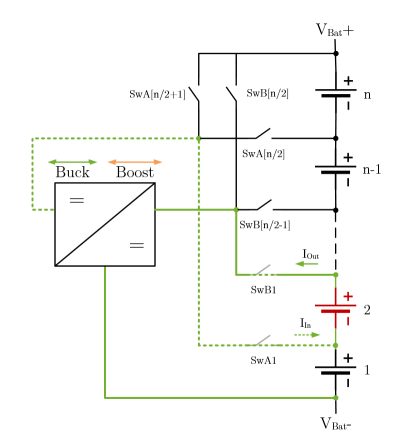
\includegraphics[width=.6\textwidth]{Chap04/Figures/Type2abABMS.PNG}
	\caption{\textit{Type IIb} active balancing architecture }
	\label{fig: Type2b active balancing architecture}
\end{figure}
A four-switch buck-boost converter similar to the one in Figure\ref{fig:Type2a Typical Buck boost}(b) can be used to realize the necessary bidirectional buck-boost converter. The ability to run the converter in a synchronous mode in both directions is a benefit of this design.


\subsection{\textit{Type IIIa} :  High - and low-side buck-boost converters :}
The system's implementation using high- and low-side buck-boost converters are shown in Figure \ref{fig:Type3a active balancing architecture}. Similar to \textit{Type I}, the operation involves the transfer of charge sequentially rather than simultaneously. There are two phases to the balancing process: one for the boost operation and one for the buck operation. The description is stack-to-cells-to-stack following accepted nomenclature. The high-side converter and low-side converter shouldn't work in the same direction at the same time to maintain a low average stack current throughout the two phases. To demonstrate how the high-side converter works in this example, balancing routes for \textit{Cell [n-1]} are also given in addition to \textit{Cell 2}\cite{Active_Balancing_Thesis_Raber}[p. 62].
Four converters, which can carry out the two phases concurrently, are used in an expanded version of this architecture\cite{Active_Balancing_Thesis_Raber}. There are more conceivable combinations: Another high-performance variant can be created by fusing the Type II concept with the Type III high-side converter.\\

\begin{figure}[h]
	\centering
	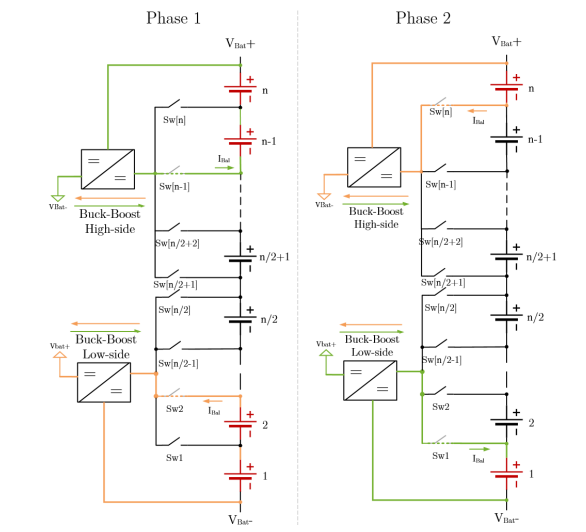
\includegraphics[width=0.6\textwidth]{Chap04/Figures/Type3a_ABMS.PNG}
	\caption{\textit{Type IIIa}  active balancing architecture}
	\label{fig:Type3a active balancing architecture}
\end{figure}
During Phase 1, the low-side converter functions as a boost converter, discharging \textit{Cells 1} and 2 through $S_{wA}$ with the converter's input current IBal, identical to Example \ref{fig:Type3a active balancing architecture}. \textit{Cell [n-1]} and \textit{Cell [n]} are simultaneously charged with IBal by the high-side converter while operating in buck mode. Phase 2 involves charging Cell 1 in buck mode and discharging \textit{Cell [n]} in boost mode to achieve the same balancing results as in Section (Results will be published in the upcoming chapters ). $I_{Bal}$ is used to charge and discharge \textit{Cell [n-1]} and \textit{Cell 2}.\\
A common ground connection allows the low-side converter to access all cells up to the middle of the battery stack, including \textit{Cell [n/2]}. It can be executed as depicted in Figure \ref{fig:Typical Schematics of the Low side and High Side buck boost Converter}. The design is made simpler by the fact that the two operating modes are only required in one direction. To enable synchronous operation for both modes, only two MOSFETs are required. If switch Q1 is not controlled, the MOSFET's intrinsic antiparallel diode enables normal operation albeit with lower efficiency.\\
The remaining cells are connected to the high-side converter through a shared $V_{Bat+}$ link. It is similar to the common ground converter in terms of design, but it has a distinct structure (see Figure \ref{fig:Type3a active balancing architecture}).
\section{Proposed Active Balancing Method}
The proposed architecture for the BMS active balancing is very similar to the \textit{type IIa and IIb} active balancing. In the proposed topologies the charge is transferred either from imbalance cell to stack or vice versa.
A bidirectional high and low-side buck-boost converter is used in the proposed architecture in place of the typical (unidirectional) buck-boost converter. Refer\ref{fig:BMS Architecture} to the Architecture to see how the switch matrix is set up to connect each battery node to the DC/DC converter's low side. The top of the battery pack is directly attached to the high side of the DC/DC converter.
\begin{figure}[h]
	\centering
	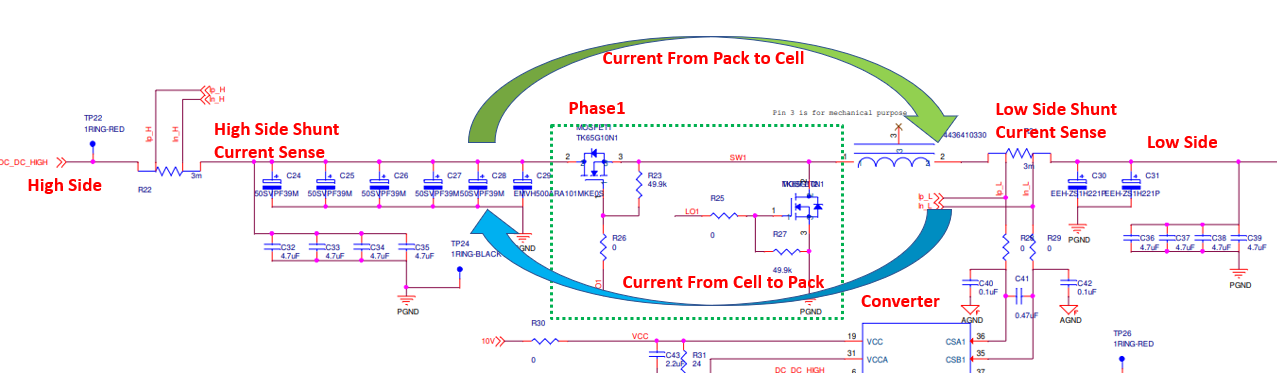
\includegraphics[width=1\textwidth]{Chap04/Figures/Low_high_side_Converter_shematic.PNG}
	\caption{Shematic of the High/Low side DC/DC converter } 
	\label{fig:High_Low_DC_DC_Shematic}
\end{figure}
The proposed architecture\ref{fig:High_Low_DC_DC_Shematic} gives more control over the balancing current that is flowing in the DC/DC controller. One of the acute advantages of the input(With High side shunt Resistance) and output current(With Low side shunt Resistance) to the DC/DC converter. The section gives a more elaborative description and technical details of this configuration.
\section{Overview of Active balancing BMS Architecture}
Figure\ref{fig:BMS Architecture} shows the overview of the Inventvm wireless BMS architecture. From the Hardware point of view, the Architecture is separated into two parts one Cell Management Unit (CMU) which sits on each battery. The other one is MMU which is on the main motherboard to control the overall functionality of the BMS. The working procedure of the architecture is as follows
\begin{figure}[h]
	\centering
	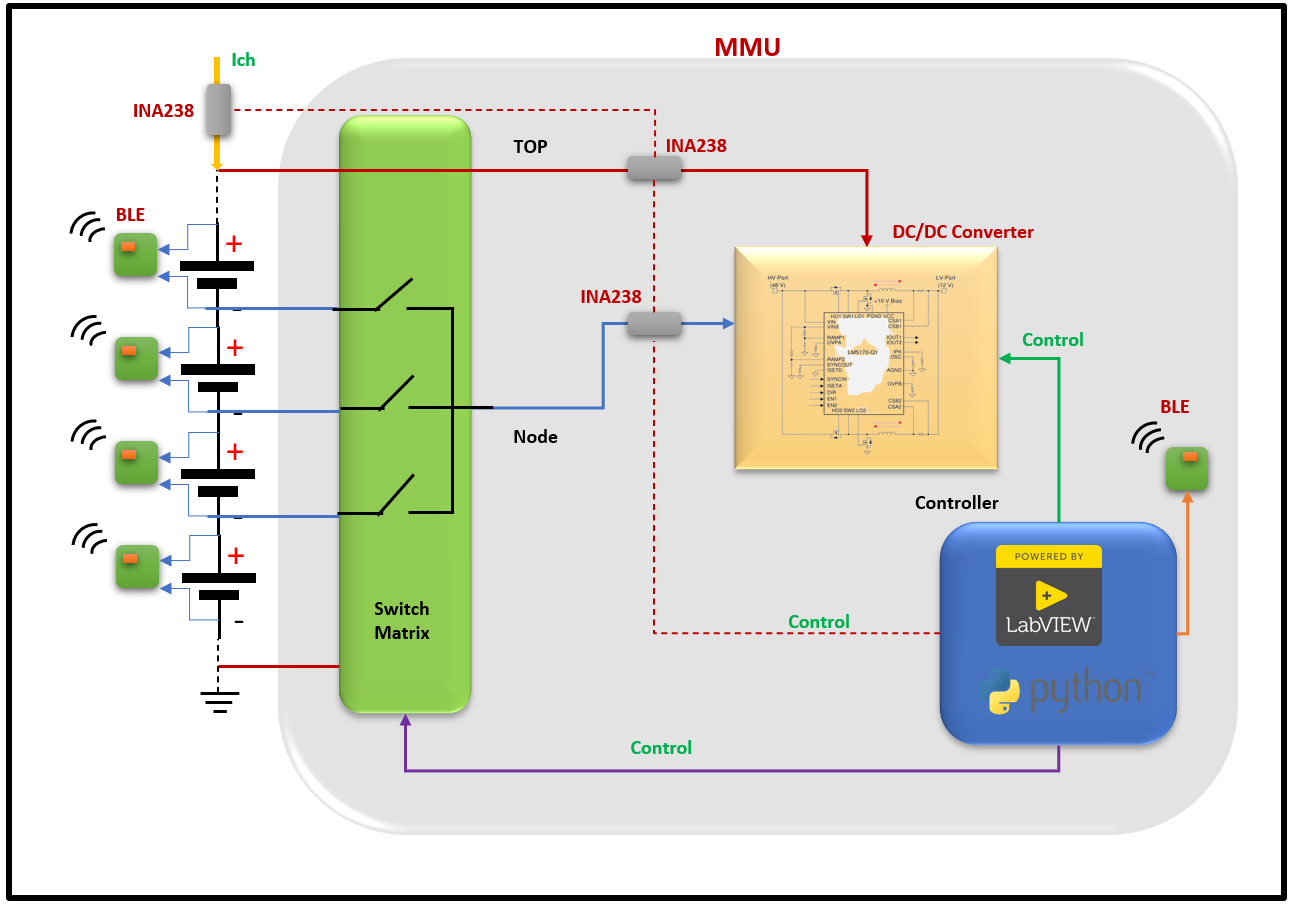
\includegraphics[width=1\textwidth]{Chap04/Figures/BMS_Architecture_border.PNG}
	\caption{BMS Architecture} 
	\label{fig:BMS Architecture}
\end{figure}
\begin{itemize}
	\item The CMUs of each battery contains Bluetooth modules, for our applications we have used BLUeNRG-355mc which will sense the live battery voltage and the temperature of the battery(using NTC).
	\item CMUs will synchronize with the master present on the MMU. According to the master request, all the CMUs Bluetooth will send the data to the Master in the given time slot.
	\item On request of the controller, the master(BLE on MMU) will collect packets from all the slaves(CMUs) and hand over the decoded data (Voltages of the Batteries and Temperature measurements) to the Controller on the MMU.
	\item The controller in this project is the PC, it could be a microcontroller also. The controller will be responsible for running all the BMS algorithms and detecting which node needs to be balanced depending on the CMU's battery voltages.
	\item In this particular project, the controller will use LabVIEW and python to build a complete BMS model and algorithm.
	\item Through the open circuit voltage(Battery voltages) received from the CMU, the controller will calculate the initial SoC(The open circuit voltage directly proportional initial SoC of the battery "manufacturer open circuit voltage to SoC curve").
	\item Once the controller finds the imbalance node through the initial SoC estimation from the open circuit voltages of the battery, the switch matrix is switched to the imbalance node and directly connected to the low side(Output) of the DC/DC converter.
	\item Depending on the battery imbalance the controller will configure the DC/DC converter either in buck or boost mode.
	\item During the Balancing, the input and output current of the DC/DC is monitored to calculate the balancing current, if the balancing current reached the threshold the DC/DC converter current is dropped.
	\item If the batteries are charging during the balancing the charging current \textit{$I_{ch}$}(Figure \ref{fig:BMS Architecture}) is also monitored through the pack current sensor.
\end{itemize}
\section{Retrospect of BMS Hardware}
\subsubsection{Multiphase Bidirectional DC/DC Current Controller LM5170-Q1}
\indent The LM5170-q1 controller is a high precision dual channel bidirectional converter applicated in automotive 48 Volts and 12Volts dual battery systems. Depending on the Direction Signal DC/DC converter regulates the average current. The Regulated current through the DC/DC converter can be programmed by analog or Digital PWM inputs.

The LM5170-q1 has a dedicated dual channel differential current sense amplifier to monitor the current flowing through the Dc/Dc converter, which can achieve $1\%$ current sense accuracy. It has a Robust Gate driver to drive half the bridge. The Internal gate driver of the LM5170 has the capability of driving parallel MOSFET switches with a capacity of 500Watts. The synchronous diode emulation mode prevents the dc to dc converter from the negative currents and also enables the discontinuous mode of operation. This property enhances the DC/DC converter efficiency tremendously. The Controller can offer benefits of cycle-by-cycle current limitation, overVoltage protection at both low side and high side ports, Temperature protection and Mosfet failure so on...
x
\subsubsection{Matrix Switch Gate Driver :}
Modern BMS application is suffocated by the hot swapping of the Batteries for balancing. When the battery node is switched in the battery pack to balance the battery node matrix(switching circuit) the MMU will see an immense current that is flowing from the battery \cite{LTC4231_User_Datasheet}. when the switch matrix is switched to a particular node of the battery pack. The battery Node will be directly connected to the output node of the DC/DC converter (The low side of the DC/DC Converter refers to the circuit \ref{fig:Typical Bidirectional circuit of the LM5170} @low side), which will be having reservoir capacitor that will sink an immense amount of the current from the battery in very short time this will cause switching FET to burn, so it essential to switch FET very carefully. such technique is called "Hot Swap". "Hot Swap" is FET switching technique Figure\ref{fig:Mosfet_Switch_Matrix}, more often used in live power switch applications. The technique allows the gate driver circuit to monitor the current flowing through the switch circuit by the input sense resistance. By any chance Hot swap circuit doesn't allow the rapid surge of the load current in the switch circuit \cite{LTC4231_User_Datasheet}.
\paragraph{LTC4231 :}
LTC4231 is an Analog Device Inc Micro power hot-swap controller that is employed to face circuit board insertion and abrupt live power supply. An internal high-side switch driver controls the gate of an external N-channel MOSFET. Back-to-back MOSFETs can be used for reverse supply protection down to –40V \cite{LTC4231_User_Datasheet}.

The LTC4231 provides a debounce delay and allows the GATE to be ramped up at an adjustable rate. After startup, the LTC4231's quiescent current drops to 4µA during normal operation with output active. UVL, UVH, OV, and GNDSW monitor overvoltage and Undervoltage periodically, keeping total quiescent current low. Pulling SHDN low shuts down the LTC4231 and the quiescent current drops to 0.3µA.

During an overcurrent fault, the LTC4231 actively limits current while running an adjustable timer \cite{LTC4231_User_Datasheet}. The LTC4231-1 remains off after a current fault while the LTC4231-2 automatically reapplies power after a cool-down period\cite{LTC4231_User_Datasheet}.

A typical circuit diagram and the operational waveforms of the LTC4231 are described in the Figure\ref{fig: LTC4231 Application circuit and the Operational waveform}. 
For more technical details refer to the ADI LTC4231 datasheet\cite{LTC4231_User_Datasheet}.

\paragraph{Inrush Control by LTC4231 :}
In most, automotive applications keeping the inrush current low and in control is essential to avoid catastrophic damage to the switching circuits. LTC4231 takes a golden hand in controlling the inrush current by startup method (Timer Delay varying). The equations \ref{eq:LTC4321_Inrush_current} implicate the Inrush current controlled by the LTC, the Inrush current highly depends on the gate capacitance of the switch, and the output capacitance of the DC/DC capacitance (load Capacitance $C_L$). A capacitor $C_G$ of the Gate to the GND can be used to control the gate voltage slew rate for the Inrush current in the Switch.
\begin{equation}\label{eq:LTC4321_Inrush_current}
    I_{InRsush} = \frac{C_{L}}{C_{G}} \times 10\mu A
\end{equation}
\begin{figure}[h]
	\centering
	\makebox[\textwidth]{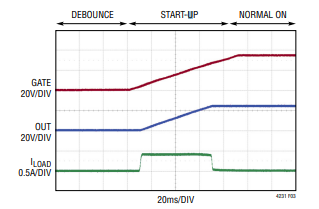
\includegraphics[width=0.9\paperwidth]{Chap04/Figures/Inrsuh_current_of_LTC4321.PNG}}
    \caption{Inrush Control by Limiting $V_{GATE}$ Slew}
    \label{fig: LTC4231 Inrush Control by Limiting VGATE Slew }
\end{figure}
The $V_{GATE}$ of the switch raise with the slope of $10\mu A/C_G$ Figure\ref{fig: LTC4231 Inrush Control by Limiting VGATE Slew}.
Once $V_{GATE}$ crosses the Vth, status goes high impedance. see the figure\cite{fig: LTC4231 Inrush Control by Limiting VGATE Slew} which explains the Inrush current protection when the $\Delta V_{Th(GATE)}$ crosses the gate voltage threshold.

The Design Example in the Chapter\ref{chap:miselleneous} explains, how to pick the design parameters to design the inrush current limit and gate driver, please follow. LTC4231 holds a wide range of advantages compared to the gate driver that is available in the market such Wide Operating Voltage Range: 2.7V to 36V, Reverse Supply Protection to –40V n Adjustable Analog Current Limit with Circuit Breaker n Automatic Retry or Latchoff on Current Fault n Overvoltage and Undervoltage Monitoring n Controls Single or Back-to-Back N-Channel MOSFETs \cite{LTC4231_User_Datasheet}. By considering all the facts we have picked the LTC4321 as the gate driver for the switch matrix.
\subsection{Current Sense :}

As elaborated in the BMS architecture High precision current sensors are used to monitor the BMS Currents. The currents are mainly monitored by the sensor charging current that is entering through the Battery pack Top and balancing current that is entering or leaving from the DC to Dc convert to the Balancing node from Battery pack TOP.

For Inventvm active balancing BMS application, The team has selected INA238 Current sensor from Texas instruments. The chapter(Current and Voltage Synchronization for BMS application) gives an extensive explanation for choosing the INA238\cite{INA238_User_Datasheet} and the application.
\subsection{Wireless Communication Hardware :}
The Bed Rock Idea behind the Inventvm active balancing BMS is to make the BMS architecture in the Wireless Communication Environment. The wireless communication architecture will reduce the immense pain of hard wires for communication in modern smart EVs. The Wireless Communication picked for the project is the Bluetooth stack, Chapter \ref{chap:BLE} takes the privilege to explain the Bluetooth Hardware choosing criteria, and design the proprietary Bluetooth solution for the projects. The BLUeNRG-355MC\cite{BLNRG355_STEVAL_GUIDE} and the Nordic\cite{NORDIC_nrf52840_USERGUIDE} are the Bluetooth solutions employed in the project.
\section{Summary of Chapter \ref{ch:Architecture_Active_Balancing_BMS}}
The initial phase of the chapter \ref{ch:Architecture_Active_Balancing_BMS} summarizes the different topologies of the BMS active balancing, more or less, many of the topologies remained on the shelf, because of the less robustness and clumsy implementation.
The proposed topology\ref{fig:High_Low_DC_DC_Shematic} for the BMS active balancing is inherited from topology \textit{Type IIa} and topology \textit{Type IIb}. Currently, by using the proposed methodology\ref{fig:High_Low_DC_DC_Shematic}, we can successfully perform the active balancing for batteries.
The active balancing BMS architecture\ref{fig:BMS Architecture} will give a much broader view in this chapter \ref{ch:Architecture_Active_Balancing_BMS}, but in this architecture\ref{fig:BMS Architecture}, I have not discussed how to calculate the SoC and SoH but following Chapters(SoC and SoH calculation chapter not yet updated) will give more extravagance on the SoC and SoH calculation and synchronization methods of the voltage and current. I have succeeded in explaining most of the BMS hardware except the current sensors because I have dedicated a separate chapter to explaining the current acquisition and synchronization(Current and Voltage synchronization chapter not yet updated) of the measurements.